\section{モデルと識別可能性}
\label{part:model}

本章ではまず、本論文で用いる数学記号を導入し、
非巡回有向グラフ(Directed Acyclic Graph, DAG)モデルとその識別可能性を定義する。
その後、本論文の提案モデルを構成する2つの既存モデルについて概説する。
既存モデルの1つ目は、連続変数を扱うDAGモデルで、
Shimizu \textit{et al.}(2006)\cite{Shimizu2006-yu}によって提案された
線形非ガウス非巡回モデル(Linear Non-Gaussian Acyclic Model; LiNGAM)である。
2つ目は、主に離散変数を扱うDAGモデルで、
Park and Raskutti(2017)\cite{Park2017-hw}によって提案された
2次分散関数(Quadratic Variance Function, QVF)DAGモデルである。
QVF-DAGモデルの識別可能性は、Park and Raskutti(2017)\cite{Park2017-hw}によって
過分散スコアを用いて証明されたが、
本論文ではPark and Park(2019)\cite{Park2019-qy}が提案した
モーメント比スコアを拡張することで、識別可能条件の緩和を行う。
最後に、連続変数と離散変数が混合したデータにおけるDAGモデルを提案し、
その識別可能性について議論する。

%
%!TEX root = ../thesis.tex

\subsection{数学的準備}

グラフは頂点(node)の集合$V=\{1,2,\dots,p\}$と、
頂点同士をつなぐ辺(edge)の集合$E\subset V \times V$ によって、
$G=(V,E)$と表現される。
グラフの辺は有向辺(矢線)と無向辺(双方向矢線)に分けることができ、
2つの頂点$j,k\in V$において、
$(j,k)\in E$かつ$(k,j)\notin E$のとき、$j$から$k$への矢線があるという。
これを$j \rightarrow k$と表現することもある。
一方で、$(j,k)\in E$かつ$(k,j)\in E$のとき、$j$と$k$の間に双方向矢線があるという。
すべての辺が有向辺であるグラフを有向グラフ(directed graph)という。
本論文では、特に断りのない限り、頂点$j$から$k$への矢線がある場合、
$j$が$k$の原因であるといった因果関係があることを表すとする。
つまり、本論文で扱うグラフにおける矢線の有無は因果関係の有無を表しており、
矢線の始点が原因で、矢線の終点が結果である。
このような定性的な因果関係を表すグラフを因果グラフ(causal graph)という。
また、グラフ$G$からすべての矢印を取り除くことによって得られるグラフを
$G$のスケルトンという。

頂点の系列$\alpha_1, \alpha_2, \dots, \alpha_{n+1}$について、
すべての$i=1,2,\dots, n$で、
$\alpha_i \rightarrow \alpha_{i+1}$、または$\alpha_{i+1} \rightarrow \alpha_i$となる矢線がある時、
長さ$n$の道(path)という。
特に、すべての$i=1,2,\dots, n$で、$\alpha_i \rightarrow \alpha_{i+1}$となる矢線がある時、
長さ$n$の有向道(directed path)という。
また、長さ$n$の有向道で、$\alpha_1 = \alpha_{n+1}$となるものを巡回閉路(cycle)という。
一方で、巡回閉路のない有向グラフは非巡回的(acyclic)であるという。
本論文では、非巡回有向グラフ(Directed Acyclic Graph; DAG)のみを扱う。

頂点$j$から$k$への矢線がある時、$j$を$k$の親(parent)といい、$k$を$j$の子(child)という。
また、$(j,k)\in E$であるすべての頂点$j$からなる集合を$Pa(k)$と表記する。
頂点$j$から$k$への有向道がある時、$j$を$k$の祖先(ancestor)、
$k$を$j$の子孫(descendant)という。
頂点$k$のすべての祖先からなる集合を$An(k)$、すべての子孫からなる集合を$De(k)$と表記する。
また、すべての頂点から$k$と$k$の子孫を除いたものを、$k$の非子孫(non-descendant)といい、
その集合を$Nd(k) \equiv V \backslash (\{k \} \cup De(k))$と表記する。
さらに、因果的順序(causal oredering)について定義する。
因果的順序とは、その順序に従って変数を並び替えると、
すべての矢線$(j,k)\in E)$について、$k$が$j$の原因になることがない順序のことであり、
$\pi =(\pi_1, \dots, \pi_p)$と表記する。
DAGで表現される因果グラフには、このような順序が(一意とは限らないが)存在するという特徴がある。
つまり、因果グラフを同定することは、因果的順序を同定することとスケルトンを同定することという
2つの工程に分解することができる。

有向グラフ$G$における頂点上の標本空間$\mathcal X_V$の確率分布に従う
確率変数の集合$X \equiv (X_j)_{j \in V}$について考える。
ここで、確率変数ベクトル$X$は、同時確率密度関数$f_G(X)=f_G(X_1, X_2, \dots, X_p)$で与えられていると仮定する。
$V$の任意の部分集合$S$について、$X_S \equiv \{X_j:j\in S \subset V \}$と
$\mathcal X_S \equiv \times_{j \in S} \mathcal X_j$を定義する。
ただし、$\mathcal X_j$は$X_j$の確率空間である。
また、任意の頂点$j\in V$について、
確率変数ベクトル$X_S$を与えたときの変数$X_j$の
条件付き確率を$f_j(X_j|X_S)$と表記する。
すると、DAG $G$によるモデルは以下のように因数分解することができる\cite{Pearl2009-oh}。

\begin{equation}
  f_G(X)=f_G(X_1, X_2, \dots, X_p) = \prod_{j=1}^p f_j(X_j | X_{Pa(j)})
  \label{eq:factorization}
\end{equation}

ここで、$f_j(X_j | X_{Pa(j)})$は、$X_j$の
親変数$X_{Pa(j)} \equiv \{ X_k:k\in Pa(j) \subset V \}$を与えた条件付き確率である。

また、本論文では観察データから因果グラフを同定するという問題を扱うため、
因果グラフの識別可能性について定義する。
識別可能性を直感的に説明すると、条件付き確率分布$f_j(X_j|X_{Pa(j)})$に対してある仮定を置くと、
同時確率密度関数$f_G(X)$を与えたDAG $G$の構造を一意に決定付けることができるということである。

識別可能性について詳細に定義するために、すべての$j \in V$に関する
条件付き確率分布$f_j(X_j|X_{Pa(j)})$の集合を$\mathcal P$と表記する。
また、グラフ$G=(V,E)$について、グラフ$G$に関する同時分布のクラスと、
分布$\mathcal P$のクラスを以下で定義する。

\begin{equation}
  \mathcal F(G;\mathcal P) \equiv \{ f_G(X) = \prod_{j \in V} f_j(X_j|X_{Pa(j)}) ;
  \text{where} f_j(X_j|X_{Pa(j)}) \in \mathcal P \quad \forall j \in V \}
\end{equation}

続いて、$p$個の変数からなる非巡回的有向グラフの集合を$\mathcal G_p$と表記する。
そこで、DAG $\mathcal G_p$の空間上の確率分布のクラス$\mathcal P$における
識別可能性を以下のように定義する。

\begin{df}[識別可能性]
  条件付き分布のクラス$\mathcal P$が$\mathcal G_p$において識別可能であるとは、
  $G,G' \in \mathcal G_p$において$G \neq G'$であるならば、
  $f_G = f_{G'}$を満たすような$f_G \in \mathcal F(G; \mathcal P)$と
  $f_G' \in \mathcal F(G'; \mathcal P)$が存在しないことである。
\end{df}

%
%!TEX root = ../thesis.tex

\subsection{LiNGAM}

本節では、連続変数データから因果構造を推定するモデルとして、
LiNGAM\cite{Shimizu2006-yu}について概説する。

LiNGAMは、観測データがDAGによって表現されるデータ生成過程から生成されるものと仮定する。
$p$個の観測変数$X = \{X_1, \dots, X_p \}$に対するLiNGAMは以下のように書ける。

\begin{equation}
  X_j = e_j + b_{j0} + \sum_{k \in Pa(j)} b_{jk}X_j
  \quad \text{with} \quad e_j \sim \text{non-Gaussian}
  \label{eq:lingam}
\end{equation}

各観測変数$X_j$は、その変数以外の観測変数$X_k$とその誤差変数$e_j$の線形和である。
また、それぞれの係数$b_{jk}$は、変数$X_k$から変数$X_j$への直接的な因果効果の大きさを表す。
加えて、誤差変数$e_j$はすべて平均0、分散非ゼロの非ガウス分布に従う連続確率変数であり、
お互いに独立であることを仮定する。
つまり、潜在交絡変数が存在しないことを仮定する\cite{Spirtes2000-mf}。

LiNGAMはShimizu \textit{et al.}(2006)\cite{Shimizu2006-yu}によって、
因果グラフとグラフを構成するパラメータが一意に識別可能であることが証明されている。

%
%!TEX root = ../thesis.tex

\subsection{2次分散関数 (QVF) DAGモデル}

本節では、主に離散変数を扱うDAGモデルとして、
Park and Raskutti(2017)\cite{Park2017-hw}によって提案された
2次分散関数 (QVF) DAGモデルについて概説する。
QVF-DAGモデルは、各頂点の親による条件付き分布$\mathcal P$の分散が、
期待値の2次式で与えられているというモデルであり、
以下のように定義される。

\begin{df}[QVF-DAGモデル\cite{Park2017-hw}]
2次分散関数(Quadratic variance function, QVF)DAGモデルは、
各頂点の親による条件付き確率分布が、
以下で表現される2次分散関数性(quadratic variance function property)を
満たすようなDAGモデルである。

すべての$j \in V$について、以下を満たすような$\beta_{j0}, \beta_{j1} \in \mathbb R$が存在する。
  \begin{equation}
      \mathrm{Var}(X_j|X_{Pa(j)}) = \beta_{j0} E(X_j | X_{Pa(j)}) + \beta_{j1} E(X_j | X_{Pa(j)})^2
      \label{QVF}
  \end{equation}
\end{df}

2次分散関数性を満たす確率分布のクラスには、
ポアソン分布、二項分布、負の二項分布、ガンマ分布などが含まれることが知られている。
これらの確率分布における$\beta_0, \beta_1$を表\ref{table:beta}に示す。

\begin{table}[ht]
  \begin{center}
    \caption{2次分散関数性を満たす確率分布における$\beta_0, \beta_1$の例}
    \begin{tabular}{llcc} \toprule
      確率分布     & $\mathcal{P}$                  & $\beta_0$ & $\beta_1$       \\ \midrule
      ポアソン分布  & $\text{Poisson}(\lambda)$      & 1         & 0               \\
      二項分布     & $\text{Binomial}(N, p)$        & 1         & $-\frac{1}{N}$   \\
      負の二項分布  & $\text{NegativeBinomial}(R,p)$ & 1         & $\frac{1}{R}$    \\
      ガンマ分布   & $\text{Gamma}(\alpha, \beta)$   & 0         & $\frac{1}{\alpha}$ \\ \bottomrule
    \end{tabular}
    \label{table:beta}
  \end{center}
\end{table}

DAGモデルにおいては、各頂点の分布がその頂点の親変数の影響を受けており、
各頂点の条件付き期待値は、任意の単調で微分可能な
リンク関数$g_j \colon \mathcal X_{Pa(j)} \rightarrow \mathbb R^+$によって、
$E(X_j|X_{Pa(j)}) = g_j(X_{Pa(j)})$で表現される。
本論文の後半では、各頂点間の関係について線形性を仮定するため、
QVF-DAGモデルのリンク関数$g_j$がパラメータに関して線形であることを仮定した
QVF構造方程式モデル(structural quation model, SEM)を導入する。

\begin{equation}
  g_j(X_{Pa(j)}) = g_j \left(\theta_j + \sum_{k \in Pa(j)} \theta_{jk}X_k \right)
\end{equation}

ここで、$(\theta_{jk})_{k \in Pa(j)}$は親変数の重み付け係数である。
例えば、ある頂点の条件付き確率分布がポアソン分布の場合、
$g_j(X_{Pa(j)}) = \exp(\theta_j + \sum_{k \in Pa(j)} \theta_{jk}X_k)$
となる。

より一般的には、指数分布族の定義を用いて、以下のように表現することができる。
\begin{equation}
  P(X_j|X_{Pa(j)}) = \exp \left( \theta_{j}X_j  + \sum_{(k,j)\in E} \theta_{jk}X_k X_j -
  B_j(X_j) - A_j \left( \theta_{j} + \sum_{(k,j) \in E} \theta_{jk} X_k \right) \right)
\end{equation}

ここで、$A_j(\cdot)$は対数分配関数(log-partition function)、
$B_j(\cdot)$は指数分布族によって決まる関数、
$\theta_{jk}\in \mathbb R$は頂点$j$に対応するパラメータである。
DAGモデルの因数分解~\eqref{eq:factorization}により、QVF-SEMの同時確率分布は、
以下のように記述することができる。

\begin{equation}
  P(X) = \exp \left( \sum_{j\in V} \theta_{j}X_j + \sum_{(k,j)\in E} \theta_{jk}X_k X_j
  - \sum_{j \in V} B_j(X_j) - \sum_{j \in V} A_j
  \left( \theta_{j} + \sum_{(k,j)\in E} \theta_{jk} X_k \right)\right)
  \label{eq:QVF_factorization}
\end{equation}

このモデルは、関数$A_j(\cdot)$や$B_j(\cdot)$が頂点$j$によって異なることを許容するため、
各条件付き分布がそれぞれ異なる分布に従っているような混合DAGモデルを表現することも可能である。
また、各頂点の分布$\mathcal P$が式~\eqref{QVF}で定義される2次分散関数性を満たす場合、
非線形モデルやノンパラメトリックモデルに拡張することも可能である。

%
%!TEX root = ../thesis.tex

\subsection{QVF-DAGモデルの識別可能性}

本節ではQVF-DAGモデルが識別可能であることを証明する。
QVF-DAGモデルの識別可能性は
Park and Raskutti(2017)\cite{Park2017-hw}によって初めて証明されたが、
本論文ではPark and Park(2019)\cite{Park2019-qy}のアイデアを用いることにより、
識別可能条件の緩和も行う。

まず初めに、QVF-DAGモデルにおけるモーメント(積率)について
以下のような関係性が成立していることを示し、識別可能性の証明に利用する。

\begin{prop} \label{prop:MRS}
  リンク関数$(g_j(X_{Pa(j)}))_{j \in V}$が非退化であるQVF-DAGモデル~\eqref{QVF}において、
  任意の頂点$j \in V$、任意の集合$S_j \subset \mathit{Nd}(j)$に関して、
  以下のモーメント関係が成立している。
  \begin{equation}
    \frac{E(X_j^2)}
    {E \left[ \beta_0 E(X_j | X_{S_j}) + (\beta_1 + 1)E(X_j | X_{S_j})^2 \right]}
    \geq 1
    \label{eq:MRS}
  \end{equation}
  同様に、
  \begin{equation}
    E(\mathit{Var}( E(X_j | X_{Pa(j)}) | X_{S_j} )) \geq 0
  \end{equation}
  等号成立は、$S_j$が頂点$j$の親変数すべてを含むとき($Pa(j)\subset S_j$)である。
\end{prop}

\begin{proof}
  分散とモーメントの関係性と、2次分散関数性の定義を利用すると、
  2次分散関数性を満たす確率変数$X$のモーメントについて、以下の関係性が成り立つ。
  \begin{alignat*}
    \mathit{Var}(X) &= E(X^2) - E(X)^2 & \qquad & \text{分散の公式より} \\
                    &= \beta_0 E(X) + \beta_1 E(X)^2 && \text{2次分散関数性の定義より}
  \end{alignat*}
  よって、
  \begin{equation*}
    E(X^2) &= \beta_0 E(X) + (\beta_1 + 1) E(X)^2
  \end{equation*}

  ここで、記号の簡単のために、$f(\mu) = \beta_0 \mu + (\beta_1 + 1)\mu^2$と関数を定義する。
  すると、任意の頂点$j \in V$、任意の空でない集合$S_j \subset \mathit{Nd}(j)$について、
  以下のように書ける。
  \begin{equation}
    \begin{split}
      E(X_j^2 | S_j) &= E(E(X_j^2 | X_{Pa(j)}) | S_j) \\
                     &= E(f(E(X_j | X_{Pa(j)})) | S_j)
      \label{moment_related}
    \end{split}
  \end{equation}

  イェンセンの不等式と関数$f(\cdot)$が凸であることを利用すると、以下が導ける。
  \begin{equation}
    \begin{split}
      E(f(E(X_j | X_{Pa(j)})) | S_j) & \geq
      f(E(E(X_j | X_{Pa(j)}) | S_j)) \\
      &= f(E(X_j | S_j))
      \label{Jensen}
    \end{split}
  \end{equation}

  ここで、モデルの定義より、$E(X_j | X_{Pa(j)}) = g_j(X_{Pa(j)})$であり、
  関数$g_j(\cdot)$は非退化であることを利用すると、
  等号は$S_j$が頂点$j$の親変数すべてを含むとき
  ($Pa(j) \subset S_j \subset \mathit(Nd)(j)$)のみ成立する。

  式~\eqref{moment_related}と式~\eqref{Jensen}を整理すると、
  \begin{equation*}
    \begin{split}
      E(X_j^2 | S_j) - f(E(X_j | S_j)) & \geq 0 \\
      E(X_j^2 | S_j) - \bigl( \beta_0 E(X_j | S_j) +
      (\beta_1 + 1) E(X_j | S_j)^2 \bigl) & \geq 0
    \end{split}
  \end{equation*}
  となり、
  さらに期待値を取ることで、
  \begin{equation*}
    E(X_j^2) - E\bigl( \beta_0 E(X_j | S_j) +
    (\beta_1 + 1) E(X_j | S_j)^2 \bigl) & \geq 0
  \end{equation*}
  が得られる。 よって、以下が成り立つ。
  \begin{equation*}
    \frac{E(X_j^2)}
    {E\bigl( \beta_0 E(X_j | S_j) + (\beta_1 + 1) E(X_j | S_j)^2 \bigl)}
    \geq 1
  \end{equation*}

  ここからは、$E(X_j^2) \geq E\bigl( \beta_0 E(X_j | S_j) +
  (\beta_1 + 1) E(X_j | S_j)^2 \bigl)$ が、
  $E(\mathit{Var}( E(X_j | X_{Pa(j)}) | X_{S_j} )) \geq 0$と
  同値であることを証明する。
  \textcolor{red}{分散の公式を用いると… ここ書く…}
  \qed

\end{proof}

直感的な理解を得るために、各頂点の親変数による条件付き確率分布がポアソン分布である
2変数DAGモデルを例にその識別可能性を証明する。
そこで、図\ref{fig:ex_bivariate}のようなDAGモデルを考える。

\begin{itemize}
  \item $G_1 \colon X_1 \sim \mathtext{Poisson}(\lambda_1),
         \quad X_2 \sim \mathtext{Poisson}(\lambda_2) \quad$ ただし、$X_1$と$X_2$は独立

  \item $G_2 \colon X_1 \sim \mathtext{Poisson}(\lambda_1),
         \quad X_2|X_1 \sim \mathtext{Poisson}(g_2(X_1))$

  \item $G_3 \colon X_2 \sim \mathtext{Poisson}(\lambda_2),
         \quad X_1|X_2 \sim \mathtext{Poisson}(g_1(X_2))$

  ただし、$g_1$と$g_2$は非退化な任意の関数である。
  $(g_1, g_2 \colon \mathbb{N} \cup \{ 0 \} \rightarrow \mathbb{R}^+)$
\end{itemize}

\begin{figure}[h]
  \centering
  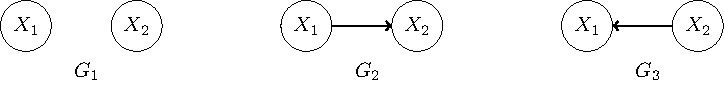
\includegraphics{./picture/bivariate.pdf}
  \caption{2変数のDAGモデル}
  \label{fig:ex_bivariate}
\end{figure}

命題\ref{prop:MRS}より、$G_1$におけるすべての頂点$j \in \{ 1,2 \}$について、
$E(X_j^2) = E(X_j) + E(X_j)^2$である。
$G_2$においては、以下が成り立つ。
\begin{equation*}
  E(X_1^2) = E(X_1) + E(X_1)^2, \quad \text{and} \quad
  E(X_2^2) > E(X_2) + E(X_2)^2
\end{equation*}
同様に、$G_3$においては、以下が成り立つ。
\begin{equation*}
  E(X_1^2) > E(X_1) + E(X_1)^2, \quad \text{and} \quad
  E(X_2^2) = E(X_2) + E(X_2)^2
\end{equation*}
つまり、モーメント比$E(X_j^2) / (E(X_j) + E(X_j)^2)$によって、
真のグラフ構造を同定することが可能である。

命題\ref{prop:MRS}のモーメント比を用いる方法は、
一般的な$p$変数のQVF-DAGモデルにも適用することが可能であり、
モーメント比~\eqref{eq:MRS}が1か1以上かを確かめることで識別可能性を証明することができる。

\begin{theo}[QVF-DAGモデルの識別可能性]
  2次分散関数性を満たす係数$(\beta_{j0}, \beta{j1})_{j=1}^p$が存在し、
  QVF-DAGモデル\eqref{eq:factorization}のクラスについて考える。
  任意の頂点$j \in V$について、$\beta_{j1} > -1$であり、
  リンク関数$g_j(\cdot)$が非退化であるならば、
  QVF-DAGモデルは識別可能である。
\end{theo}

\begin{proof}
  一般性を失わずに、真の因果順序が一意であり、$\pi = (\pi_1, \dots, \pi_p)$であると仮定する。
  また、簡単のために、$X_{1:j} = (X_{\pi_1}, X_{\pi_2}, \dots, X_{\pi_j})$、
  $X_{1:0} = \emptyset$と定義する。
  加えて、モーメント関連関数$f(\mu) = \beta_0 \mu, (\beta_1 + 1)\mu^2$を定義する。

  ここからは数学的帰納法を用いてQVF-DAGモデルの識別可能性を証明する。

  \textbf{Step(1)}
  因果順序が最初である$\pi_1$について、
  命題\ref{prop:MRS}を用いると、
  $E(X_{\pi_1}^2) = E(f(E(X_{\pi_1})))$であるのに対し、
  任意の頂点$j \in V \backslash \{ \pi_1 \}$については、
  $E(X_j ^2) > E(f(E(X_j)))$である。
  よって、因果順序が1番目の要素$\pi_1$を特定することができる。

  \textbf{Step(m-1)}
  因果順序が$(m-1)$番目の要素について、
  因果順序が先の$m-1$個の要素とその親が正しく推定されていると仮定する。

  \textbf{Step(m)}
  因果順序が$m$番目の要素とその親について考える。
  命題\ref{prop:MRS}より、$\pi_m$は、
  $E(X_{\pi_m}^2) = E(f(E(X_{\pi_m} | X_{1:(m-1)})))$である。
  一方で、$j \in \{ \pi_{m+1}, \dots, \pi_p \}$については、
  $E(X_j^2) > E(f(E(X_j | X_{1:(m-1)})))$である。
  よって、因果順序が$m$番目の要素$\pi_m$を推定することができる。

  親変数に関しては、$P(G)$の因数分解\eqref{eq:factorization}による
  以下の条件付き独立関係より導くことができる。
  \begin{align*}
    E(X_{\pi_m}^2) &= E(f(E(X_{\pi_m} | X_{1:(m-1)}))) \\
                   &= E(f(E(X_{\pi_m} | X_{Pa(\pi_m)})))
  \end{align*}
  つまり、上記の関係が成立するような最小の集合を
  $X_{1:(m-1)}$の中から$\pi_m$の親として選択することができる。

\qed
\end{proof}

Park and Raskutti(2017)\cite{Park2017-hw}によって証明された
QVF-DAGモデルの識別可能条件には、
$Pa(j) \nsubseteq S_j$のとき、すべての$x \in \mathcal X_{S_j}$について、
$\mathit{Var}(E(X_j | X_{Pa(j)}) | X_{S_j} = x) > 0$という
仮定が含まれていた。
しかし、本論文における識別可能条件にはそのような仮定は含まれていない。
つまり、従来の識別可能条件\cite{Park2017-hw}を緩和している。
この識別可能条件の緩和によってPoisson-SEMの学習が容易になることが、
Park and Park(2019)\cite{Park2019-qy}の3.2節において議論されている。

%
%!TEX root = ../thesis.tex

\subsection{提案モデル}

本節ではLiNGAM \cite{Shimizu2006-yu}とQVF-DAGモデル\cite{Park2017-hw}を
組み合わせることによって、
連続変数と離散変数の両方から構成されるDAGモデルを提案する。

